%! Author = joels
%! Date = 27/01/2022

\section{Virtual Machine}
\begin{minipage}{0,4\linewidth}
    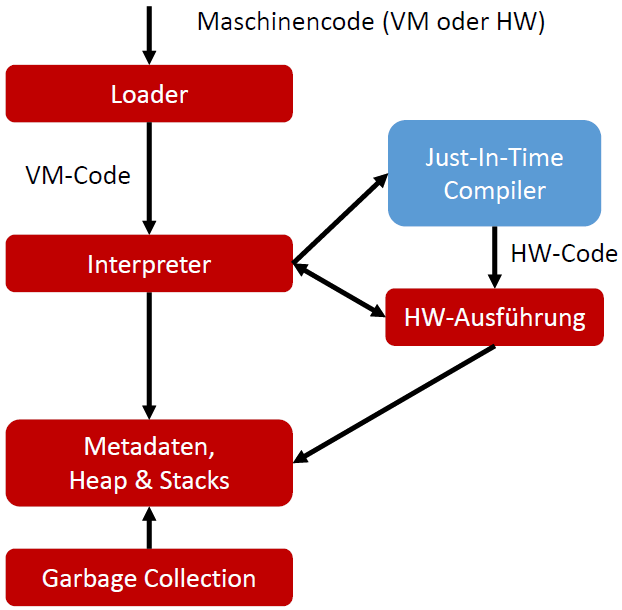
\includegraphics[width=\linewidth]{aufbau_laufzeitsystem}
\end{minipage}
\begin{minipage}{0,6\linewidth}
    \subsection{Loader}
    \begin{itemize}[topsep=0pt]
        \itemsep -0.2em
        \item Lädt Zwischencode (File) in Speicher
        \item Alloziert Speicher
        \SubItem{Metadaten für Klassen, Methoden, Variablen, Code}
        \item Definiert Layouts
        \SubItem{Speicherbereiche für Fields/Variablen/Parameter}
        \item Address Relocation
        \SubItem{Löst Verweise auf zu Methoden, Typen, anderen Assemblies}
        \item Initiiert Programmausführung
        \SubItem{Interpreter oder Compilation (JITer)}
        \item Optional: Verifier zum erkennen von falschem IL-Code oder anderen Fehlern (Stack over/underflow, Typefehler, illegaleSprünge etc.)
        \SubItem{Sonst: Überprüfunfen zur laufzeit (unser Approach)}
    \end{itemize}
\end{minipage}

\subsubsection{Deskriptoren}
Laufzeitinfo für Typen \& Methoden:
\begin{itemize}[topsep=0pt]
    \itemsep -0.2em
    \item Typen: Klassen, Arrays oder Basistypen
    \item Klassen: Field-Typen
    \item Methoden: Typen von Parameter \& Locals, Rückgabetyp, Bytecode
\end{itemize}
\textbf{Zusätzlich gut zum merken:} Parent Klasse, Virtual Method Table\\
\begin{minipage}{0,5\linewidth}
    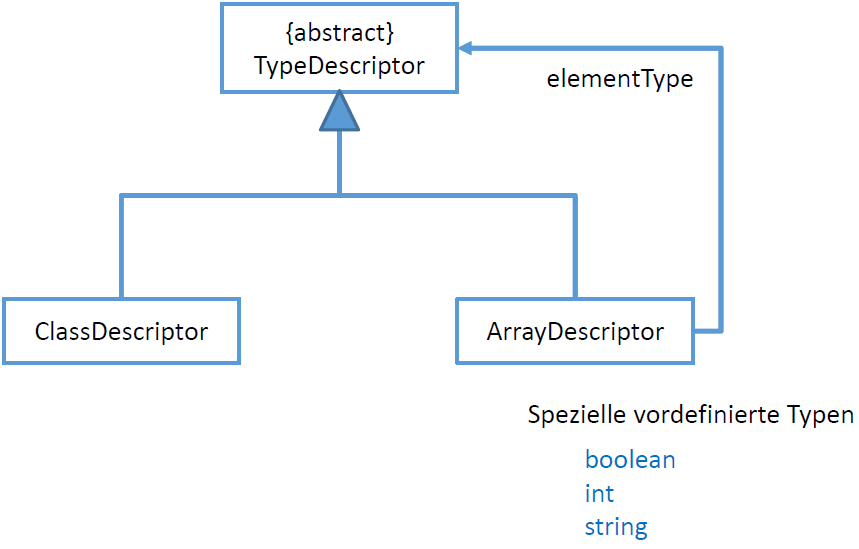
\includegraphics[width=\linewidth]{type_descriptor}
\end{minipage}
\begin{minipage}{0,5\linewidth}
    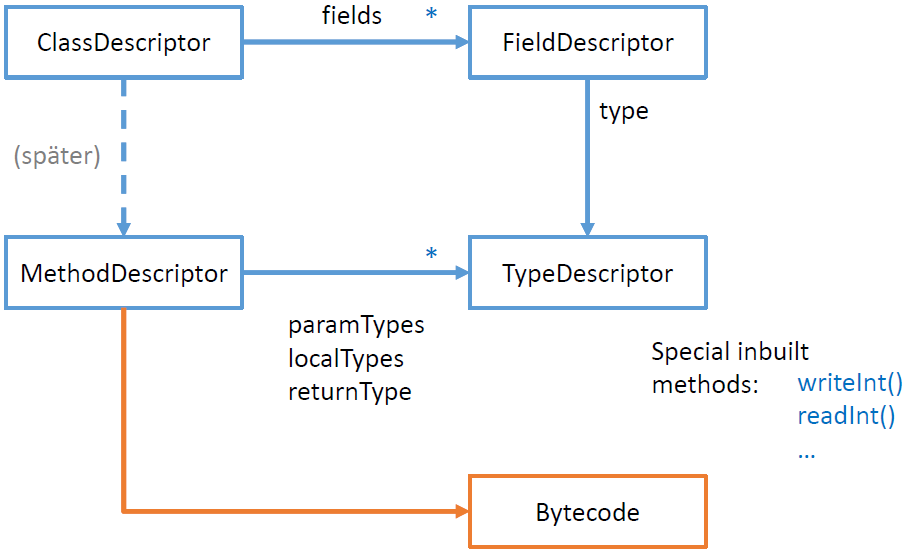
\includegraphics[width=\linewidth]{method_class_descriptor}
\end{minipage}

\subsubsection{VM: Managed \& Unmanaged}
Da wir für die VM Java verwenden kriegen wir Managed Runtime Support. Wir wollen aber einen eigenen GC bauen.\\
$\rightarrow$ Kleine Unmanaged Teile neben der Java VM: Heap und HW-Execution (JIT).

\subsection{Interpreter}
\begin{itemize}[topsep=0pt]
    \itemsep -0.2em
    \item Interpreter Loop
    \SubItem{Emuliert Instruktion nach der anderen}
    \item Instruction Pointer (IP)
    \SubItem{Adresse der nächsten Instruktion}
    \item Evaluation Stack
    \SubItem{Für virtuellen Stack Prozessor}
    \item Locals \& Parameters
    \SubItem{Für aktive Methode}
    \item Method Descriptor
    \SubItem{Für aktive Methode}
\end{itemize}

\subsubsection{Ausführung}
\begin{lstlisting}
// execute() emuliert Instruktion je nach Op-Code
switch(instruction.getOpCode()){
    case LDC -> push(instruction.getOperand());
    case IADD -> {
        var right = pop();
        var left = pop();
        var result = left + right;
        push(result);
    }
}
\end{lstlisting}

\subsubsection{Prozedurale Unterstützung}
\begin{itemize}[topsep=0pt]
    \itemsep -0.2em
    \item Methodenaufrufe
    \SubItem{invokevirtual = Aufruf neuer Methode}
    \SubItem{return = Rücksprung aus Methode}
    \item Activation Frame
    \SubItem{Datenraum einer Methode}
    \SubItem{Parameter, lokale Variablen, temporäre Auswertungen}
    \item Call Stack
    \SubItem{Stack der Activation Frames gemäss Aufrufreihenfolge}
\end{itemize}
\textbf{Call Stack Design:}\\
Managed Call Stack im Interpreter. Unmanaged bei HW-Execution

\subsection{Gesamtbild}
\begin{minipage}{0.5\linewidth}
    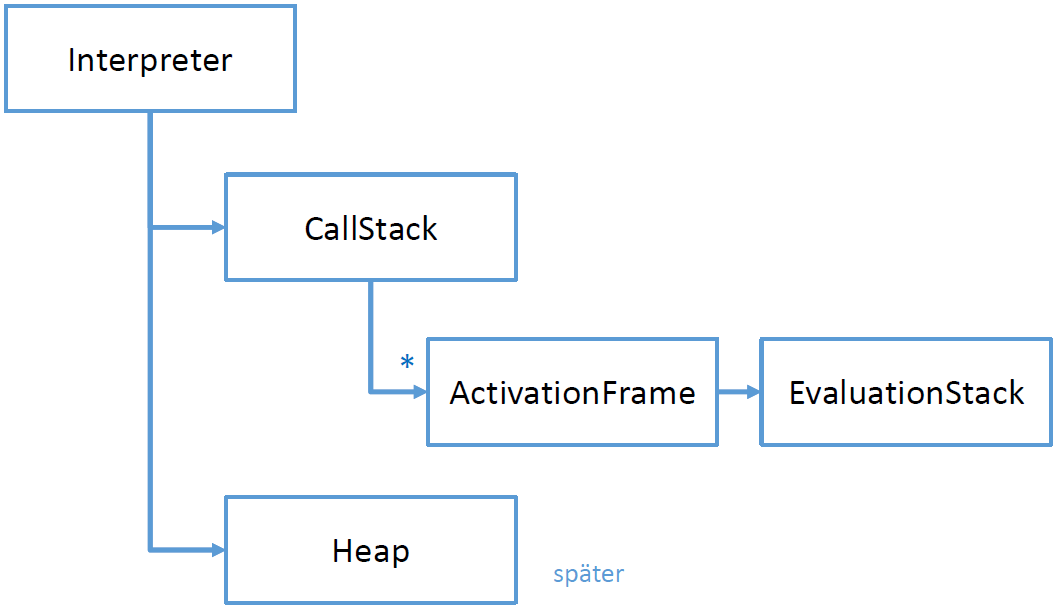
\includegraphics[width=\linewidth]{laufzeitsystem_gesamtbild}
\end{minipage}
\begin{minipage}{0.5\linewidth}
    \textbf{Verifikation im Interpreter}
    \begin{itemize}[topsep=0pt]
        \itemsep -0.2em
        \item Korrekte Benutzung der Instruktionen
        \SubItem{Typen stimmen (bei Operatoren, Aufrufen etc.)}
        \SubItem{Methodenaufrufe stimmen (Argumente, Rückgabe etc.)}
        \SubItem{Sprünge sind gültig}
        \SubItem{Op-Codes stimmen}
        \item Typen sind bekannt
        \SubItem{Metadaten (Typen der Fields/Locals/Parameters)}
        \SubItem{Werte auf Evaluation Stack haben Typ}
    \end{itemize}
\end{minipage}

\textbf{Sicherheitsmassnahmen}
\begin{itemize}[topsep=0pt]
    \itemsep -0.2em
    \item Korrekter Bytecode und Typenkonsistenz prüfen
    \item Variablen immer initialisieren (auch lokale)
    \item Checks durchführen (Null, Array-Index etc.)
    \item Stack Overflow und Underflow Detections
    \item Kompatibilität von externen Verweisen (hier nicht)
    \item Garbage Collection
\end{itemize}

\textbf{Interpreter vs Kompilation}
\begin{itemize}[topsep=0pt]
    \itemsep -0.2em
    \item Interpreter ist ineffizient
    \SubItem{Dafür aber flexibler und einfach zu entwickeln}
    \SubItem{Akzeptabel für selten ausgeführten Code}
    \item Kompilierter HW-Prozessor Code ist schneller
    \SubItem{JIT Compilation für Hot Spots}
    \SubItem{Kompilation kostet, Laufzeit macht es (allenfalls) wett}
\end{itemize}